\chapter{Methodology}
\label{chapter:methodology}

This chapter first introduces the technology stack chosen that this project will be built upon in section \ref{section:llvm}, then discuss the two core methodologies used by the project, class hierarchy tree reconstruction, and object-flow analysis, in section \ref{section:class-tree} and section \ref{section:object-flow} respectively. Finally, evaluation of the work is discussed in section \ref{section:evaluation}.

\section{LLVM}
\label{section:llvm}

LLVM is a compiler and toolchain technologies framework \cite{llvm-website} composed of a collection of projects, most notably are

\begin{itemize}
    \item Clang, an optimizing C/C++/Objective-C compiler
    \item LLVM Core, a set of libraries offering architecture independent optimization and code generation support for different CPU architectures
\end{itemize}

These components are designed to work closely with \ac{llvm-ir}, an architecture and programming language independent form of software programs. It is similar to assembly language, in the sense that a piece of program in LLVM IR form is also composed of instructions that have operations and operands, but LLVM IR is portable across different CPU architectures, and preserves certain high-level language information, such as strong types and functions \cite{llvm-ir}.

\begin{figure}[H]
    \centering
    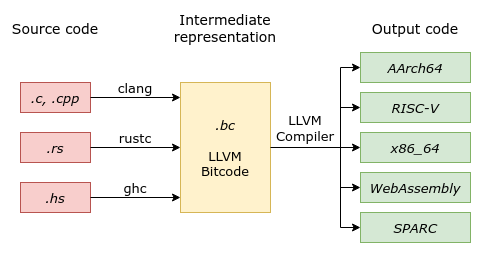
\includegraphics[keepaspectratio,width=0.6\paperwidth]{img/llvm-compiler.png}
    \caption{LLVM Compiling Pipeline \cite{llvm-pipeline}}
    \label{fig:llvm-compiler}
\end{figure}

\begin{figure}[H]
    \centering
    \begin{lstlisting}[language=c]
double square(double num) {
    return num * num;
}
    \end{lstlisting}
    \begin{lstlisting}[language=llvm]
define dso_local double @_Z6squared(double %0) local_unnamed_addr #0 {
  %2 = fmul double %0, %0
  ret double %2
}
    \end{lstlisting}
    \begin{lstlisting}[language={[x86masm]Assembler}]
square:
    sub     esp, 12
    movsd   xmm0, qword ptr [esp + 16]
    mulsd   xmm0, xmm0
    movsd   qword ptr [esp], xmm0
    fld     qword ptr [esp]
    add     esp, 12
    ret
    \end{lstlisting}
    \caption{a C++ function, its LLVM IR, and its x86 assembly code}
    \label{fig:llvm-ir}
\end{figure}

Figure \ref{fig:llvm-compiler} shows the process of compiling a program from source code to a binary executable that is runnable on a target architecture in LLVM. The compiler, Clang for C/C++ programs or \texttt{rustc} for Rust programs, takes source code as input, parses the syntax and semantics of the program, and emits LLVM IR code in a binary file format called LLVM bitcode (\texttt{.bc}). LLVM backend (annotated as ``LLVM Compiler'' in the graph) then generates assembly code for the target architecture from the LLVM bitcode produced in the previous step.

Figure \ref{fig:llvm-ir} illustrates an example of a C++ function being compiled to LLVM IR and x86 assembly code. In LLVM IR, program constructs including function prototype, function name\footnote{Function name becomes \texttt{\_Z6squared} instead of the original \texttt{square} because of C++ name mangling \cite{name-mangling}.}, function body, and type of operands in each instruction, are fully preserved. In contrast, these information are mostly lost in x86 assembly code.

The project plans to implement the analysis program on top of the LLVM framework. The analysis is to be performed on LLVM IR which is stored in LLVM bitcode files. The subject program to be analyzed needs to be compiled to LLVM bitcode first, and then the analysis program loads and reads these \texttt{.bc} LLVM bitcode files.

Compared to directly analyzing the compiled binary in target architecture machine code, LLVM IR preserves much more information about constructs of the program, most importantly it keeps type information of functions, parameters, variables and operands. This is greatly beneficial to class hierarchy tree reconstruction and object-flow analysis, which are discussed in section \ref{section:class-tree} and \ref{section:object-flow} respectively.

\newpage

\section{Class Hierarchy Tree Reconstruction}
\label{section:class-tree}

Class hierarchy tree reconstruction refers to recovering information of C++ class inheritance information from LLVM IR, so that the scope of possible target functions of a class method invocation can be refined.

\begin{figure}[H]
    \centering
    \begin{lstlisting}[language=c++]
// Super class
class Animal {
    public:
        virtual std::string Name() { return "Animal"; }
};

// Derived from Animal, overrides Name()
class Pet : public Animal {
    public:
        std::string Name() override { return "Pet"; }
};

// Derived from Pet, overrides Name() again
class Dog : public Pet {
    public:
        std::string Name() override { return "Dog"; }
};
    \end{lstlisting}
    \caption{An example C++ class hierarchy}
    \label{fig:class-hierarchy}
\end{figure}

\begin{figure}[H]
    \centering
    \begin{lstlisting}[language=c++]
void funcA(Pet *object) {
    std::cout << object->Name() << std::endl;
}

void funcB() {
    Pet *object = new Dog;
    funcA(object);
    delete object;
}
    \end{lstlisting}
    \caption{Calling class methods}
    \label{fig:class-caller}
\end{figure}

In Figure \ref{fig:class-hierarchy}, the superclass \texttt{Animal} has a method \texttt{Name}. Class \texttt{Pet} inherits from class \texttt{Animal} and overrides method \texttt{Name}. Class \texttt{Dog} inherits from class \texttt{Pet} and overides method \texttt{Name} again.

When analyzing the function body of \texttt{funcA()} in Figure \ref{fig:class-caller}, with class inheritance relationship information, it can be deduced that the possible target functions of \texttt{object->Name()} can only be either \texttt{Pet::Name()} or \texttt{Dog::Name()}, but absolutely not \texttt{Animal::Name()}. This is because \texttt{object} is of type \texttt{Pet}, and \texttt{Animal} is neither the class \texttt{Pet} itself nor its subclass, so \texttt{Animal::Name()} must not be a target function.

This motivating example demonstrates that class hierarchy tree reconstruction can help eliminate overridden superclass methods from the possible target function set of a class method call. Compared to simple function prototype matching, this technique can greatly narrow down the target function set when the type of the caller object is relatively deep and closer to leaf nodes in the class hierarchy tree, because all the virtual method implementations belonging to its superclasses and sibling classes are filtered out, despite having the same function prototype (\texttt{void(void)}).

A possible approach to implement class hierarchy tree reconstruction from LLVM IR is analyzing virtual table of classes to find out class inheritance relationships. Each class type has a static virtual table that is shared by all instances of classes of this single type. Clang compiler organizes virtual tables in the layout \cite{type-metadata} \cite{vtable} shown in Table \ref{tab:vtable-layout}. The second entry in the virtual table points to the \ac{rtti} table of the class. \ac{rtti} table contains a pointer to the string representing class type name \cite{vtable}, as well as entries pointing to \ac{rtti} tables of parent classes. This information can be used to determine parent-descendant class inheritance relationships. Appendix \ref{appendix:vtable} presents an example of virtual table in LLVM IR.

\begin{table}[H]
    \centering
    \begin{tabular}{|c|c|}
        \hline
         Offset & Meaning \\
        \hline \hline
         0 & ``\texttt{offset-to-top}'' \\
        \hline
         1 & address to \acs{rtti} \\
        \hline
         2 & address to first method \\
        \hline
         \dots & \dots \\
        \hline
    \end{tabular}
    \caption{Layout of a virtual table}
    \label{tab:vtable-layout}
\end{table}

\section{Object-Flow Analysis}
\label{section:object-flow}

Object-flow analysis takes a step further in refining target function set of a class method call. It analyzes what concrete types that a class object in a function can possibly take, by keeping track of assignment and loading operations on the variable.

In Figure \ref{fig:class-caller}, in \texttt{funcB()}, although pointer \texttt{object} is declared with the type of \texttt{Pet}, it is assigned with a \texttt{Dog} instance at line 6, and is passed as parameter to \texttt{funcA()}. Assuming \texttt{funcA()} is only called from \texttt{funcB()} in the entire program, it can be deduced that the only type \texttt{object} can actually take in \texttt{funcA()} is \texttt{Dog}. Hence the target function set of method call \texttt{object->Name()} at line 2 in \texttt{funcA()} can be refined to only contain \texttt{Dog::Name()}.

A possible approach to implement object-flow analysis is iterative search. Starting with an initial set of possible concrete types an object can take, it follows the logic flow of the program and detects if there is any value assignments to the object. There could be an instance of another concrete type assigned to the object. If this happens, add the new concrete type to the set. Repeat the process, until the set is stabilized, i.e., no more type can be added to the set.

\section{Evaluation}
\label{section:evaluation}

After the implementation of the analysis program is completed, it will be trialled on real-world large scale C++ projects, such as Chromium, an open source web browser engine with around 12 million lines\footnote{Data from around August 2019 \cite{chromium-loc}.} of C++ code.

The performance of the analysis program developed in the project, as well as the target functions resolution results produced, will be analyzed and compared to other previous approaches in resolution of target functions of function pointers, such as type matching and multi-layer type analysis described in section \ref{section:type-analysis} and section \ref{section:mlta} respectively.

\section{Summary}
\label{section:methodology-summary}

This chapter discusses the methodology applied in the project. In the next chapter, current project status is presented.